\newcommand{\descriereIdempotenta}{Termenul 'idempotenta' este folosit pentru a evidentia faptul ca o parte dintre operatiile efectuate de catre mecanismul automatizat de generare a infrastructurii vor avea acelasi rezultat daca vor fi apelate de mai multe ori. Din motive de securitate, unele operatii vor fi definite explicit ca nefiind idempotente (e.g. generarea de chei de acces pentru API-ul 'Surf', generarea adresei de acces a API-ului (nu va fi suprascrisa in API-ul existent)) }

Procesul de generare a infrastructurii (engl. 'deployment') consta in crearea resurselor si pornirea sistemelor necesare pentru ca web-crawler-ul 'Surf' sa functioneze. Mecanismul de generare a resurselor executa urmatorii pasi:

\begin{itemize}

	\item{Crearea entitatilor necesare in AWS (e.g. functii Lambda, roluri IAM, API-ul APIGateway etc.);}
	
	\item{Stabilirea relatiilor intre resurse si injectarea dependentelor (e.g. unei rute a API-ului trebuie sa ii fie asociat un rol IAM care sa ii permita invocarea unei functii Lambda);}
	
	\item{Generarea SDK-ului Javascript necesar pentru a putea invoca API-ul 'Surf' din cadrul clientului web;}
	
	\item{Generarea unui fisier de configurare injectabil in clientul web 'Surf' pentru a stabili parametrii interactiunii intre client si cloud-ul AWS (e.g. regiunea AWS in care s-a generat infrastructura, metadate legate de rolurile utilizatorilor, cheia generata pentru a restrictiona accesul asupra API-ului etc.).}

\end{itemize}

Efortul necesar pentru generarea infrastructurii este mare, datorita complexitatii inerente a proiectului. Efectuarea manuala a pasilor in interfata web AWS (engl. 'AWS Web Console`) necesita foarte mult timp si este predispusa la erori. De asemenea, asigurarea disponibilitatii crawler-ului in mai multe regiuni globale AWS sau pe mai multe conturi AWS ar necesita repetarea identica a pasilor enumerati mai sus, pentru fiecare astfel de regiune sau cont. De aceea, crawler-ul web 'Surf' pune la dispozitie o modalitate automatizata de deployment, configurabila, testabila si reutilizabila, asigurand idempotenta\footnote{\descriereIdempotenta} la nivelul efectuarii operatiilor in cadrul AWS.

Mecanismul automatizat de generare a infrastructurii AWS reprezinta un program care primeste, ca date de intrare, un fisier de configurare in format JSON, genereaza resursele AWS si ofera clientului web, ca date de iesire, prin injectarea dependentelor, informatii si mecanisme pentru utilizarea infrastructurii create. Cerintele pentru executia cu success a deployment-ului, precum si validitatea resurselor generate reprezinta existenta credentialelor AWS necesare pentru pasii de deployment (e.g. IAM 'administrator-access') si generarea pachetului (.jar) care sa contina codul functiilor Lambda care se doresc a fi incarcate in AWS. Mai jos se poate observa un exemplu de fisier de configurare pentru generatorul de resurse AWS 'Surf':

\begin{figure}[ht]
\begin{minted}{json}
{
  "awsAccountId": "011759591962",
  "awsAccessKey": "#######" // Obfuscat intentionat,
  "awsClientRegion": "eu-west-1",
  "lambdaCodePath": "../lambda/target/surf-lambda-backend-1.0-SNAPSHOT.jar",
  "lambdaRuntime": "java8",
  "apiGatewayEndpoint": "apigateway.amazonaws.com",
  "apiStageName": "v1",
  "apiStageMetricsEnabled": true,
  "apiStageThrottlingRateLimit": "5",
  "apiStageThrottlingBurstLimit": "20",
  "apiLoggingLevel": "INFO",
  "apiGeneratedSdkType": "javascript",
  "apiGeneratedSdkOutputPath": "../../frontend/generated/sdks/",
  "apiGeneratedSdkFolderName": "api-gateway-js-sdk",
  "clientConfigFilePath": "../../frontend/generated/config/aws-config.json",
  "lambdaConfigFilePath": "../lambda/generated/config/lambda-config.json",
  "dynamoDBWorkflowsTableReadCapacityUnits": "2",
  "dynamoDBWorkflowsTableWriteCapacityUnits": "2"
}
\end{minted}
\begin{center}
	\caption{Fisier de configurare (intrare) pentru generatorul de resurse}\par\medskip
	\vspace*{-20pt}
\end{center}
\end{figure}

Pentru a asigura conexiunea clientului web cu infrastructura creata, generatorul de resurse AWS injecteaza un fisier de configurare in clientul web, intr-un director special destinat acestui sens. Politicile de securitate implementate in generatorul de resurse nu vor permite suprascrierea fisierului/directorului din clientul web in cazul in care acesta exista deja, pentru a evita pierderea datelor. Un astfel de fisier de confiurare este cel prezentat in \textit{Figura 5}:
\\

\begin{figure}[ht]
\begin{minted}{json}
{
  "awsClientRegion": "eu-west-1",
  "awsAccessKey": "#######",
  "facebookWebIdentityBasicRoleArn": "arn:aws:iam::011759591962:role/fb-role",
  "apiKey": "#######"
}
\end{minted}
\begin{center}
	\caption{Fisier folosit pentru configurarea clientului}\par\medskip
	
\end{center}
\end{figure}

Diagrama din \textit{Figura 6} prezinta procesul de construire a infrastructurii, ordonand temporal pasii necesari pentru crearea si configurarea crawler-ului. Inainte de inceperea deployment-ului resurselor AWS, se genereaza o arhiva ce contine codul sursa al functiilor Lambda. Procesul incepe cu citirea fisierului de configurare si se incheie cu generarea API-ului prin care utilizatorii vor putea accesa serviciul web. Acolo unde este necesar, se specifica interdependentele intre sisteme. De exemplu, este necesar ca mai intai sa fie create functiile Lambda, inainte ca acestea sa fie inregistrate in cadrul mecanismului de notificare asincrona oferit de SNS (de aici si numarul 4 asociat generarii functiilor lambda, reprezentand o prioritate mai mare decat numarul 5 asociat serviciului SNS). Dupa finalizarea procesului de generare a infrastructurii, pasii 1 si 4 se vor executa inca odata, in contextul executiei precedente (i.e. avand la dispozitie toate referintele catre resursele create), pentru a actualiza codul functiilor Lambda in vederea accesarii resurselor mentionate.

\begin{figure}[ht]
\begin{center}
	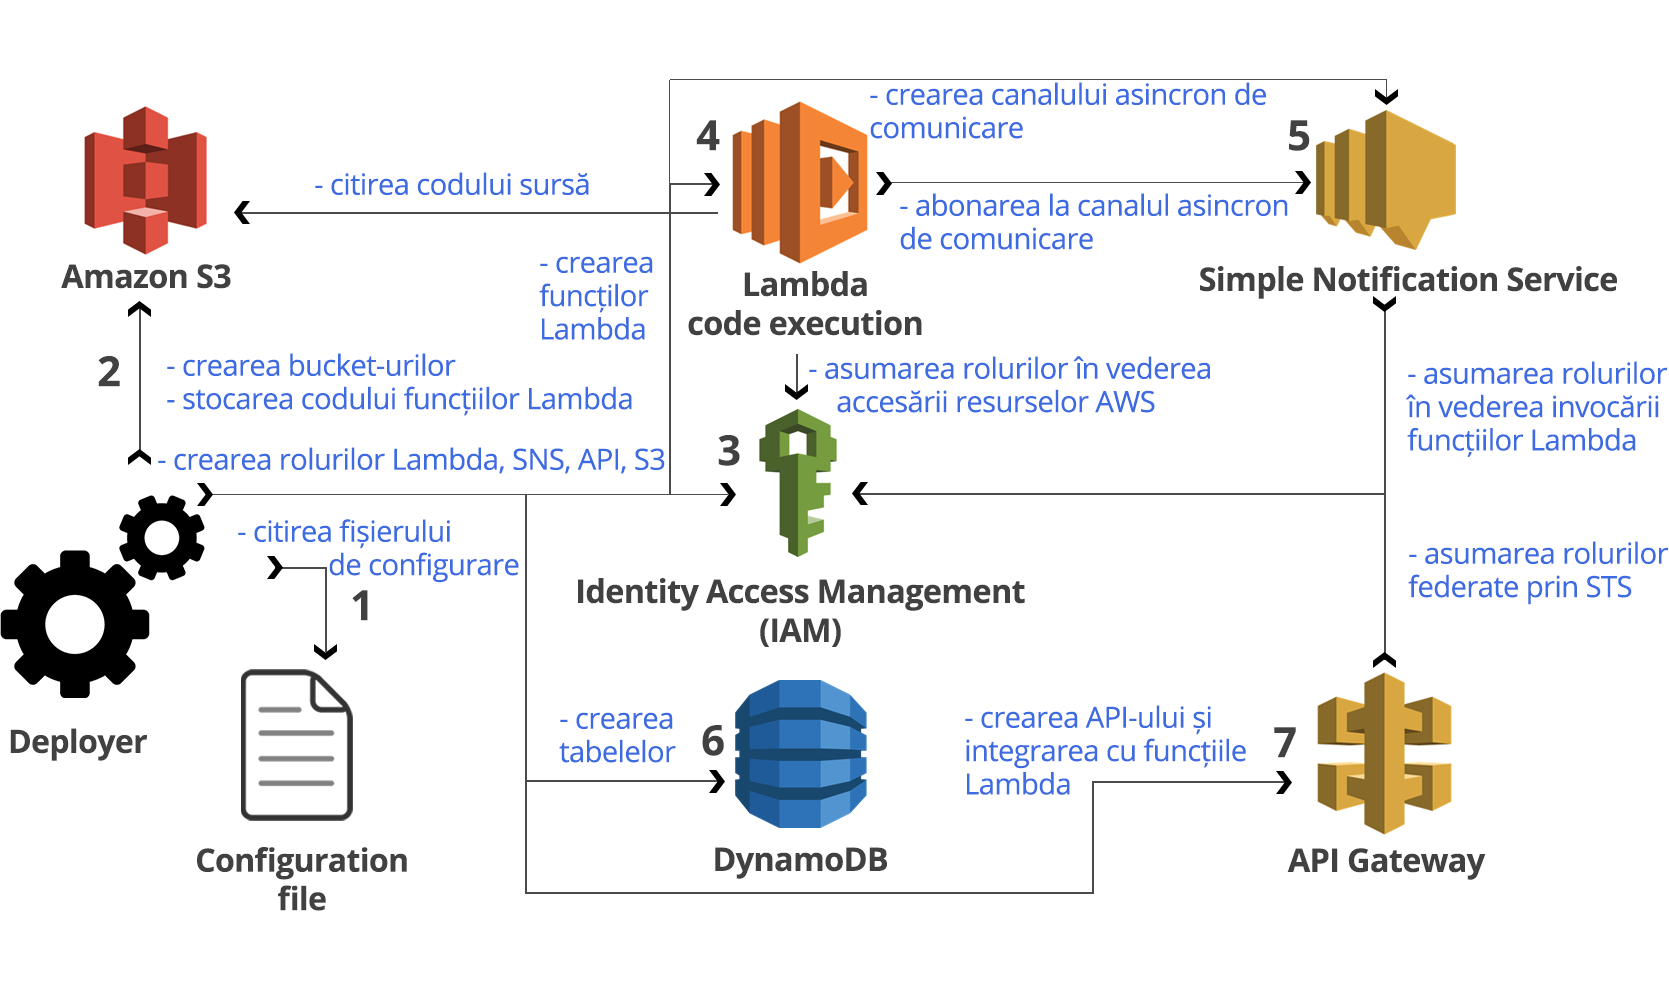
\includegraphics[keepaspectratio, width=1.0\textwidth]{generare-infrastructura.png}
	\caption{Generarea infrastructurii \cite{diagram-icons-sources}\cite{aws-icons-source}}\par\medskip 

\end{center}
\end{figure}

 